\documentclass[10pt,a4paper]{article}
\usepackage[margin=1.8cm]{geometry}
\usepackage[T1]{fontenc}
\usepackage{lmodern}
\usepackage{microtype}
\usepackage[hidelinks]{hyperref}
\usepackage{titlesec}
\titlespacing*{\section}{0pt}{0.7em}{0.25em}
\setlength{\parskip}{0.25em}
\setlength{\parindent}{0pt}
\usepackage{graphicx}
\usepackage{float}
\usepackage[font=small,labelfont=bf]{caption}
\title{\vspace{-2.4em}\textbf{ObjectSynth}: What Does This Object Sound Like?}
\author{Giovanni Nocerino \and Giacomo Cordella}
\date{\vspace{-0.8em}Software Engineering, November 2026}

\begin{document}
\maketitle
\vspace{-1.8em}

\section*{Overview}
Have you ever looked at a mug, a key, or a random gadget on your desk and wondered what it would sound like as a synth? That curiosity is where \textbf{ObjectSynth (OS)} starts. We built it for two reasons: to give a practical creative shortcut to music producers who struggle with sound design and feel stuck tweaking endless presets, and to answer a question anyone who loves music has asked at least once: what would this object actually sound like? You can run OS as a standalone playground or drop it straight into a DAW like Ableton Live or FL Studio as a VST3. Under the hood, C++ and the JUCE framework handle the plugin wrapper, the UI, and the real-time audio engine, while Python takes care of vision and signal processing: OpenCV manages the camera and visual measurements, NumPy drives the signal math (including the FFTs behind the wavetable), and Meta's Segment Anything Model (SAM 2.1, running on PyTorch via Ultralytics)~[1] carves the object out of the frame.

Splitting the project in two came naturally: \emph{Image Processing} turns what the camera sees into meaningful synth inputs, and \emph{Synth Programming} turns those numbers into something you actually want to play.

\section*{Image Processing}
Once SAM 2.1 hands us a clean binary mask of the main object in view, we had to solve two core musical problems: extracting a \textbf{waveform} to define the raw timbre, and picking \textbf{effects} that give that timbre character, possibly following natural intuition.

\textbf{Waveform Extraction.} A waveform is a 1D array of amplitude values repeated cycle after cycle, the sonic fingerprint of the sound. Starting from the photo inside SAM's 2D mask, the most direct way to get a 1D wave was to collapse one axis into the other. For a clean, readable first pass, we averaged the brightness along each column to build the cycle index by index.

\textbf{Effect Application.} OS has many parameters, and wiring image extracted features to each one of them, keeping a reasonable relation between look and sound, was not the right path. Instead, we measure six visual traits anyone can spot at a glance: sharpness (Harris corner detector), brightness (CIELAB lightness), body (share of the frame), asymmetry (overlap with a mirrored version), texture (Canny edge detector), and colourfulness (CIELAB chroma). Each trait nudges a small cluster of musically related controls with different scaling (Figure~\ref{fig:macro}). Sharp edges bite and attack fast, bright objects open up, big ones stretch wide and long, and colourful ones shimmer. A nice visualization is documented in \texttt{docs/explorer.html} inside the repository.

\section*{Synth Programming}
The synth plays up to eight notes at once and is written from scratch on top of JUCE.
Each note repeats the object's waveform at the pitch of the key, can be thickened by
detuned copies of itself, and has its own envelope and filter, so it can start with a
``pluck'' and fade like a real instrument. The notes are then summed and share a tone
filter, a distortion and a chorus.

\textbf{Per note or on the mix.} Where each module lives depends on whether it follows
each note's own timing or how the notes combine. Envelopes start with each
note, so they stay per note; a plain filter treats a sum like its parts, so it runs once
on the mix, at an eighth of the cost. Distortion is the interesting case: on the mix the
notes of a chord interact like through a guitar amplifier, which is the sound we wanted.

\textbf{Modulation and smoothness.} The LFO can move up to four knobs at once through a
small modulation matrix, without changing the values saved in the preset; filter
frequencies move in octaves, as we hear them. Every change, from a knob to a new
waveform on a held note, reaches the sound as a glide of a few milliseconds, since a
sudden jump is heard as a click.

\section*{Interesting Problems We Encountered}

\textbf{Wavetable.} Turning images into sound involves some arbitrary choices. During the experimental phase we liked two waveform extraction methods, so we decided to keep both. Inspired by Serum's (a popular synth) wavetable position control, which slices through a 3D surface of waves, we interpolated between the two waveforms so the player can sweep to whatever sweet spot fits the track (Figure~\ref{fig:wavetable}).

\begin{figure}[h]
  \centering
  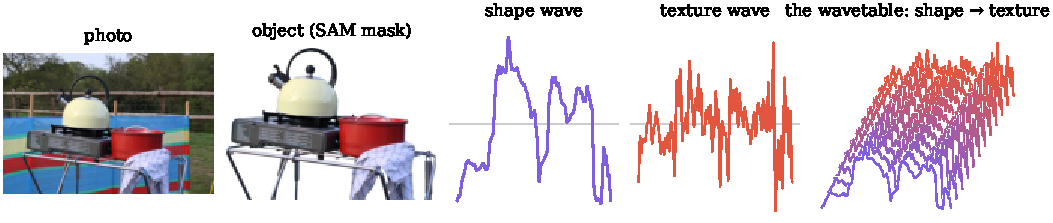
\includegraphics[width=\linewidth]{figures/teapot_strip.pdf}
  \vspace{-1.6em}
  \caption{From a photo to a wavetable: the object is cut out, read as a \emph{shape} and as a
    \emph{texture}, and the synth slides between the two waves.}
  \label{fig:wavetable}
  \vspace{-0.3em}
\end{figure}

\textbf{The LFO and the Host.} A DAW requests audio in blocks whose size the host controls. Early on, we updated the LFO once per block, which turned fast sweeps into stair-stepped jumps on large buffers and made the same project sound inconsistent across hidden host settings. Counting elapsed time in samples fixed that: the LFO now steps at a consistent rate regardless of buffer size. That fix also surfaced a subtler bug (notes triggering early or repeatedly), which we caught by enforcing a straightforward invariant: a chord played together must match the sum of its notes played one by one.

\textbf{The Nyquist Frequency.} Early prototypes overlooked a classic digital audio trap: frequencies above half the sample rate cannot be represented cleanly. High notes started sounding rough and slightly out of tune; checking the pitch revealed upper harmonics crossing Nyquist and folding back as aliasing. Now each waveform stores band-limited versions with fewer harmonics, and every voice plays the version that is safe for its pitch.

\textbf{Limitations.} Mapping pixels to sound will always be a creative design choice rather than ground truth: two sound designers would wire the same object differently. Lighting, cluttered backgrounds, and mask accuracy also still affect the result more than we would like.


\begin{figure}[H]
  \centering
  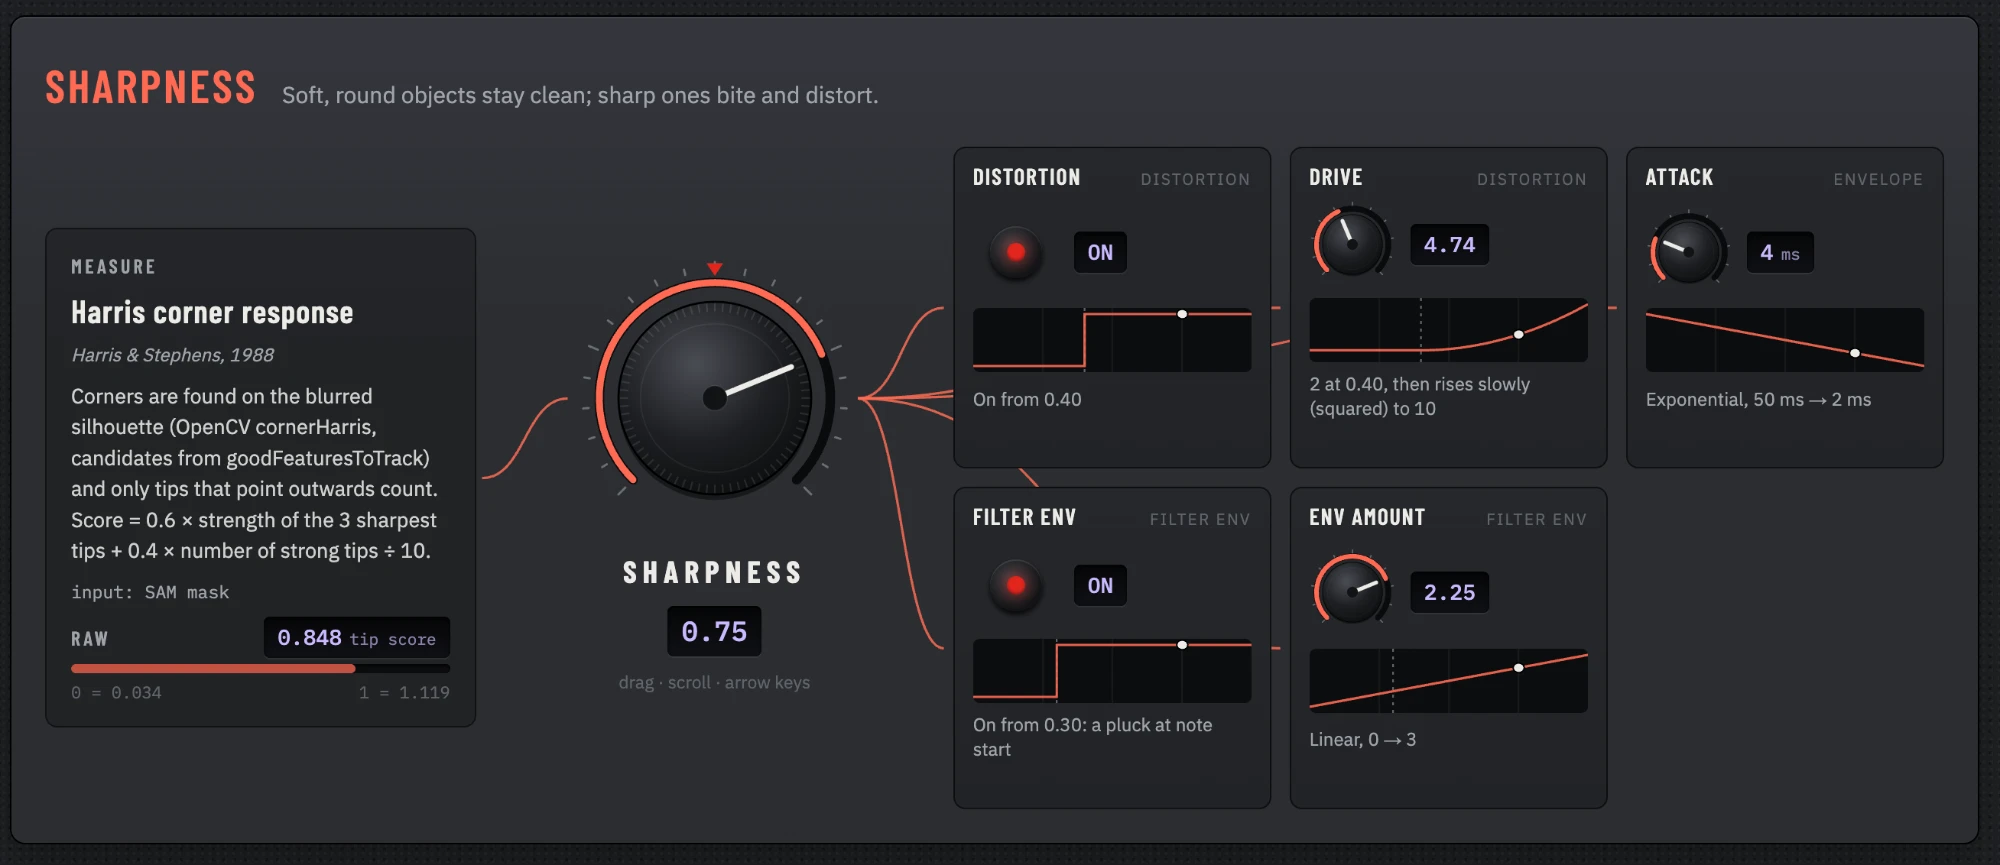
\includegraphics[width=\linewidth]{figures/macro.png}
  \vspace{-1.4em}
  \caption{An example of how a macro works: the Harris corner response sets the sharpness, which turns distortion, drive, attack and the filter envelope.}
  \label{fig:macro}
  \vspace{-0.8em}
\end{figure}

\vspace{0.2em}
{\small [1] N.~Ravi et al. \emph{SAM 2: Segment Anything in Images and Videos}, 2024. \url{https://arxiv.org/abs/2408.00714}}

\end{document}
